\documentclass[12pt]{article}
\usepackage[left=1cm, right=1cm, top=2cm,bottom=1.5cm]{geometry} 

\usepackage[parfill]{parskip}
\usepackage[utf8]{inputenc}
\usepackage[T2A]{fontenc}
\usepackage[russian]{babel}
\usepackage{enumitem}
\usepackage[normalem]{ulem}
\usepackage{amsfonts, amsmath, amsthm, amssymb, mathtools}
\usepackage{tabularx}
\usepackage{hhline}

\usepackage{accents}
\usepackage{fancyhdr}
\pagestyle{fancy}
\renewcommand{\headrulewidth}{1.5pt}
\renewcommand{\footrulewidth}{1pt}

\usepackage{graphicx}
\usepackage[figurename=Рис.]{caption}
\usepackage{subcaption}
\usepackage{float}

%%Наименование папки откуда забирать изображения
\graphicspath{ {./images/} }

%%Изменение формата для ввода доказательства
\renewcommand{\proofname}{$\square$  \nopunct}
\renewcommand\qedsymbol{$\blacksquare$}

%%Изменение отступа на таблицах
\addto\captionsrussian{%
	\renewcommand{\proofname}{$\square$ \nopunct}%
}
%% Римские цифры
\newcommand{\RN}[1]{%
	\textup{\uppercase\expandafter{\romannumeral#1}}%
}

%% Для удобства записи
\newcommand{\MR}{\mathbb{R}}
\newcommand{\MC}{\mathbb{C}}
\newcommand{\MQ}{\mathbb{Q}}
\newcommand{\MN}{\mathbb{N}}
\newcommand{\MTB}{\mathbb{T}}
\newcommand{\MTI}{\mathbb{I}}
\newcommand{\MI}{\mathrm{I}}
\newcommand{\MJ}{\mathrm{J}}
\newcommand{\MH}{\mathrm{H}}
\newcommand{\MT}{\mathrm{T}}
\newcommand{\MU}{\mathcal{U}}
\newcommand{\MV}{\mathcal{V}}
\newcommand{\MB}{\mathcal{B}}
\newcommand{\MW}{\mathcal{W}}
\newcommand{\ML}{\mathcal{L}}
\newcommand{\VN}{\varnothing}
\newcommand{\VE}{\varepsilon}

\theoremstyle{definition}
\newtheorem{defn}{Опр:}
\newtheorem{rem}{Rm:}
\newtheorem{prop}{Утв.}
\newtheorem{exrc}{Упр.}
\newtheorem{lemma}{Лемма}
\newtheorem{theorem}{Теорема}
\newtheorem{corollary}{Следствие}

\newenvironment{cusdefn}[1]
{\renewcommand\thedefn{#1}\defn}
{\enddefn}

\DeclareRobustCommand{\divby}{%
	\mathrel{\text{\vbox{\baselineskip.65ex\lineskiplimit0pt\hbox{.}\hbox{.}\hbox{.}}}}%
}
%Короткий минус
\DeclareMathSymbol{\SMN}{\mathbin}{AMSa}{"39}
%Длинная шапка
\newcommand{\overbar}[1]{\mkern 1.5mu\overline{\mkern-1.5mu#1\mkern-1.5mu}\mkern 1.5mu}
%Функция знака
\DeclareMathOperator{\sgn}{sgn}

%Функция ранга
\DeclareMathOperator{\rk}{\text{rk}}

%Обозначение константы
\DeclareMathOperator{\const}{\text{const}}

\DeclareMathOperator*{\dsum}{\displaystyle\sum}
\newcommand{\ddsum}[2]{\displaystyle\sum\limits_{#1}^{#2}}

%Интеграл в большом формате
\DeclareMathOperator{\dint}{\displaystyle\int}
\newcommand{\ddint}[2]{\displaystyle\int\limits_{#1}^{#2}}
\newcommand{\ssum}[1]{\displaystyle \sum\limits_{n=1}^{\infty}{#1}_n}

\newcommand{\smallerrel}[1]{\mathrel{\mathpalette\smallerrelaux{#1}}}
\newcommand{\smallerrelaux}[2]{\raisebox{.1ex}{\scalebox{.75}{$#1#2$}}}

\newcommand{\smallin}{\smallerrel{\in}}
\newcommand{\smallnotin}{\smallerrel{\notin}}

\newcommand*{\medcap}{\mathbin{\scalebox{1.25}{\ensuremath{\cap}}}}%
\newcommand*{\medcup}{\mathbin{\scalebox{1.25}{\ensuremath{\cup}}}}%

\makeatletter
\newcommand{\vast}{\bBigg@{3.5}}
\newcommand{\Vast}{\bBigg@{5}}
\makeatother

%Промежуточное значение для sup\inf, поскольку они имеют разную высоту
\newcommand{\newsup}{\mathop{\smash{\mathrm{sup}}}}
\newcommand{\newinf}{\mathop{\mathrm{inf}\vphantom{\mathrm{sup}}}}

%Скалярное произведение
\DeclarePairedDelimiterX{\inner}[2]{\langle}{\rangle}{#1, #2}

%Подпись символов снизу
\newcommand{\ubar}[1]{\underaccent{\bar}{#1}}

%% Шапка для букв сверху
\newcommand{\wte}[1]{\widetilde{#1}}

%%Функция для обозначения равномерной сходимости по множеству
\newcommand{\uconv}[1]{\overset{#1}{\rightrightarrows}}


\begin{document}
\lhead{Математический анализ - \RN{3}}
\chead{Шапошников С.В.}
\rhead{Лекция - 12}
\section*{Компактность}

\begin{defn}
	Если $\forall \VE > 0$ множество имеет конечную $\VE$-сеть, то оно называется \uwave{вполне ограниченным}.
\end{defn}

\begin{theorem}(\textbf{критерий компактности Хаусдорфа})
	Пусть $(X,\rho)$ - полное метрическое пространство. Множество $K \subset X$ - компакт $\Leftrightarrow K$ - замкнуто и вполне ограниченно.
\end{theorem}

\begin{theorem}(\textbf{критерий компактности в} $B(X)$)
	Множество $K \subset B(X)$ - компакт $\Leftrightarrow$ верно следующее:
	\begin{enumerate}[label={\arabic*)}]
		\item $K$ - замкнуто;
		\item $K$ - ограниченно;
		\item $\forall \VE > 0, \, \exists$ разбиение $X$ на конечное число множеств $X_1, \dotsc, X_N$ $\left(X = \bigsqcup\limits_{n = 1}^N X_n \right)$ такое, что:
		$$
		\forall f \in K, \, \forall i, \, \forall y,z \in X_i, \, |f(y) - f(z)| < \VE
		$$
		то есть на каждом из этих кусочков ($X_i$) все функции одинаково мало меняют свое значение;
	\end{enumerate}
\end{theorem}

\begin{theorem}(\textbf{Арцела-Асколи})
	Множество $K \subset C[a,b]$ компактно $\Leftrightarrow$ 
	\begin{enumerate}[label={\arabic*)}]
		\item $K$ - замкнуто;
		\item $K$ - \uwave{равномерно ограниченно}, то есть: 
		$$	
			\exists \, C > 0 \colon \forall f \in K, \, \|f\| \leq C
		$$
		\item $K$ - \uwave{равностепенно непрерывно}, то есть: 
		$$
			\forall \VE > 0, \, \exists \, \delta > 0 \colon \forall f \in K, \, \forall x,y \in [a,b],\,  |x - y| < \delta \Rightarrow  |f(x) - f(y)| < \VE
		$$
	\end{enumerate}
\end{theorem}
\begin{rem}
	Равностепенная непрерывность это усиление свойства равномерной непрерывности. Функция непрерывная на отрезке является равномерно непрерывной, а вот теперь $\delta$ выбирается не только для всех $x,y$ но и для всех $f$.
\end{rem}
\begin{proof}\hfill\\
	($\Rightarrow$) Свойства $1)$ и $2)$ - очевидны, поскольку компакт - ограниченное и замкнутое множество. Проверим свойство $3)$. Мы знаем, что:
	$$
		\forall \VE > 0, \, \exists \, \text{конечная }\VE\text{-сеть}, \, f_1, \dotsc, f_N \in K \colon \forall f \in K, \, \exists \, k \in {1,\dotsc, N}\colon \|f - f_k\| = \max\limits_{[a,b]}|f - f_k|  <\VE
	$$
	Каждая из этих функций является непрерывной по условию $\Rightarrow$ является равномерно непрерывной: 
	$$
		\forall f_k, \, \forall \VE > 0, \, \exists \, \delta_k > 0 \colon \forall x,y \in [a,b], \, |x - y| < \delta_k \Rightarrow |f_k(x) - f_k(y)| < \VE 
	$$
	Поскольку функций конечное число, то возьмем $\delta = \min\limits_{1 \leq k \leq N}\{\delta_k\}$, тогда:
	$$
		\forall k = \overline{1,N}, \, \forall x, y \in [a,b], \, |x - y| < \delta \Rightarrow |f_k(x) - f_k(y)| < \VE 
	$$
	Возьмем произвольную функцию $f \in K$ и начнем сравнивать:
	$$
		\forall x, y \in [a,b], \, |x -y| < \delta \Rightarrow |f(x) - f(y)| \leq |f(x) - f_k(x)| + |f_k(x) - f_k(y)| + |f_k(y) - f(y)|
	$$
	выбираем $k$ таким образом, чтобы $|f(x) - f_k(x)| < \VE$ и $|f(y) - f_k(y)| < \VE$, это возможно так как, $f_k$ из $\VE$-сети. Тогда:
	$$
		|f(x) - f_k(x)| + |f_k(x) - f_k(y)| + |f_k(y) - f(y)| \leq 3\VE
	$$
	то есть равностепенная непрерывность выполняется.
	
	($\Leftarrow$) Для критерия Хаусдорфа нужно, чтобы пространство было полным (с прошлого семестра знаем, что пространство непрерывных функций на отрезке - полное, см. второй семестр, лекцию $6$, теорему $3$), нужно, чтобы множество было замкнутым (есть по условию) и вполне ограниченным, то есть существовала конечная $\VE$-сеть. 
	
	По утверждению $5$ лекции $10$, если мы построим конечную $\VE$-сеть в пространстве ограниченных функций $B[a,b], \, \forall \VE > 0$, то мы построим конечную $2\VE$-сеть уже из элементов самого множества $\Rightarrow$ построим конечную $2\VE$-сеть в пространстве непрерывных функций $C[a,b], \, \forall \VE > 0$, поскольку $C[a,b] \subset B[a,b]$ с той же самой метрикой (это одна и та же метрика для непрерывных функций). Для построения конечной $\VE$-сети (из теоремы $2$ лекции $11$) множества $K \subset B[a,b]$ воспользуемся критерием компактности:
	$$
		\forall \VE > 0, \, \exists \, \{X_1, \dotsc, X_N\} \text{ - разбиение }X \colon \forall f \in K,\,\forall i, \, \forall y,z \in X_i, \, |f(y) - f(z)| < \VE
	$$
	Заметим, что условие равностепенной непрерывности буквально дает такое разбиение отрезка. Возьмем некоторое $\VE > 0$, найдем для него $\delta > 0$ из условия $3)$ и проходим отрезок $[a,b]$ шагом меньше $\delta$. Следовательно, это и будут те самые требуемые $X_i$, поскольку:
	$$
		\forall f \in K, \, \forall i, \, \forall y,z \in X_i \Rightarrow |y - z| < \delta \Rightarrow |f(y) - f(z)| < \VE
	$$
	то есть мы получаем:
	$$
		\forall f \in K, \, \forall i, \, \forall y,z \in X_i, \,|f(y) - f(z)| < \VE
	$$
	таким образом выполняется критерий компактности $\Rightarrow$ выполняется критерий Хаусдорфа $\Rightarrow$ множество $K$ - компакт и мы получили требуемое.
\end{proof}

\subsection*{Типичный пример}
Множество 
$$
	K_{R,L} = \left\{f \in C[a,b] \colon \max\limits_{t \in [a,b]}|f(t)|\leq R \wedge |f(t) - f(s)| \leq L|t-s|\right\}
$$
это типичный компакт в пространстве непрерывных функций. $R,L$ - фиксированы.
Первое свойство: 
$$
	\max\limits_{t \in [a,b]}|f(t)|\leq R
$$ 
говорит, что это равномерно ограниченное множество. Второе свойство:
$$
	|f(t) - f(s)| \leq L|t-s|
$$
говорит, что это равностепенно непрерывное множество. Единственное, что остается проверить - замкнутость множества: содержит ли это множество пределы всех своих последовательностей? Пусть есть набор функций $\{f_n\} \colon f_n \to f$, предел в этом пространстве означает, что максимум разности стремится к нулю $\Rightarrow$ эта сходимость равномерная на $[a,b]$:
$$
	\{f_n\}\colon f_n \to f \Leftrightarrow \max\limits_{t \in [a,b]}|f_n(t) - f(t)| \to 0 \Leftrightarrow f_n \uconv{[a,b]}f
$$
Таким образом, в этом множестве взять сходящуюся последовательность это то же самое, что взять равномерно сходящуюся последовательность. Будут ли для функции $f$ выполнятся условия на $K_{R,L}$. Пусть верно:
$$
	|f_n(t)| \leq R, \,	\forall t \in [a,b] \wedge |f_n(t) - f_n(s)| \leq L |t-s|
$$
Устремим $n$ к бесконечности, поскольку у нас есть равномерная сходимость, то у нас есть и поточечная сходимость: $f_n(t) \to f(t), \, \forall t$, тогда по правилу перехода к пределу в неравенстве:
$$
	|f(t)| \leq R, \,	\forall t \in [a,b] \wedge |f(t) - f(s)| \leq L |t-s|
$$
Следовательно $f$ также принадлежит множеству $K_{R,L}$. 

\begin{defn}
	Множество \uwave{выпукло}, если с любыми $2$ своими точками содержит отрезок, их соединяющий.
\end{defn}
\begin{rem}
	Заметим, что это множество - выпуклое. Пусть $f,g \in K_{R,L}$, опишем все функции из отрезка соединяющего две данные функции:
	$$
		[f,g] = \{\alpha f + (1- \alpha)g \mid \alpha \in [0,1]\}
	$$
	Очевидно, что неравенства $K_{R,L}$ сохраняются и для этого отрезка $\Rightarrow K_{R,L}$ - выпуклый компакт. Для выпуклого компакта есть теорема Шаудера (которую сможем доказать только в следующем семестре).
\end{rem}

\begin{theorem}(\textbf{Шаудер})
	Пусть $(X, \|{\cdot}\|)$ - нормированное пространство. Пусть $K\subset X$ это выпуклый компакт в нормированном пространстве и $F \colon K \to K$ это непрерывное отображение. Тогда существует неподвижная точка:
	$$
		\exists \, x \in K \colon F(x) = x
	$$
\end{theorem}

Мы можем доказать, что для отрезка это так, но это не очевидно даже для шара (теореме Брауэра). Если взять теорему Арцела-Асколи и теорему Шаудера, позволяют в практически одно касание доказать теорему о существовании решения дифференциального уравнения.

\newpage
\section*{Существование решения задачи Коши} 
Пусть $b \in C([0,T] \times \MR_x)$ - непрерывная функция двух переменных. Рассмотрим следующую задачу:
$$
	\arraycolsep=2pt
	\left\{ 
	\begin{array}{lcl}
		\dot{x} &=& b(t,x), \, t \in [0,T] \\
		x(0) &=& x_0 
	\end{array}\right. \eqno{(*)}
$$
Это задача Коши. Когда у этой системы есть решения? В общем случае их может не быть. Для существования решения достаточно непрерывности правой части. Кроме того, если требовать непрерывной дифференцируемости по $x$, то этого будет достаточно для единственности. Пусть $|b| \leq M$.
\begin{exrc}
	Пусть $b$ - любое, можно ли построить простой пример задачи Коши у которой нет решений?
\end{exrc}
\begin{proof}
	Следующая система не имеет решений:
	$$
		\arraycolsep=2pt
		\left\{ 
		\begin{array}{lcl}
			\dot{x} &=& D(t), \, t \in [0,T] \\
			x(0) &=& x_0 
		\end{array}\right. \eqno{(*)}
	$$
	где $D(t)$ - функция Дирихле. Функция $D(0) = 1$. По теореме Дарбу не может производная у всюду дифференцируемой функции иметь два значения $0$ и $1$, потому что для производной выполняется теорема о промежуточном значении.
\end{proof}
\begin{exrc}
	Рассмотреть следующую функцию:
	$$
		\dot{x} = \begin{cases}
			-1,& x \geq 0\\
			1,&  x < 0
		\end{cases}
	$$
	Обосновать, почему у неё нет решений. 
\end{exrc}
\begin{theorem}(\textbf{Пеано})
	Если $b \in C\left([0,T] \times \MR\right), \, \forall s,x, \, |b(s,x)| \leq M$, то $\forall x_0$ задача Коши $(*)$ имеет решение.
\end{theorem}
\begin{rem}
	Заметим, что здесь не указывается единственность. Кроме того, если отказаться в теореме от ограниченности, то придется выбирать другой отрезок вместо $[0,T]$. Более того, теорема Пеано верна только в конечномерных пространствах.
\end{rem}
\begin{proof}
	Доказательство будет проходить в несколько этапов:
	\begin{enumerate}[label ={(\arabic*)}]
		\item $F \colon K_{R,M} \to K_{R,M}$;
		\item $F$ - непрерывное отображение;
		\item $F(x) = x \Leftrightarrow$ выполнены условия задачи Коши $(*)$;
	\end{enumerate}
	Пусть $R = |x_0| + MT$, рассмотрим множество:
	$$
		K_{R,M} = \{x \in C[0,T] \colon |x(t)| \leq R \wedge |x(t) - x(s)| \leq M|t-s|\}
	$$
	как мы уже доказали, по теореме Арцела-Асколи это множество является выпуклым компактом (как вполне ограниченное и замкнутое множество по критерию Хаусдорфа). Заметим, что задача Коши эквивалентна следующей:
	$$
		x \in C[0,T], \, x(t) = x_0 + \ddint{0}{t}b(s,x(s))ds 
	$$
	В одну сторону нужно просто продифференцировать (при условии непрерывности функции под интегралом), а в обратную просто проинтегрировать (см. курс дифф. ур-ний). Тогда видно какое отображение должно обладать неподвижной точкой (аргумент есть функция $x(t)$):
	$$
		F\colon x(s)\mapsto F(x)\,(t) = x_0 + \ddint{0}{t}b(s,x(s))ds   
	$$
	Пусть $x \in C[0,T]$, рассмотрим $F(x)\,(t)$. Поскольку $|b|\leq M$, $t \in [0,T]$ и $x_0$ - фиксировано, то:
	$$
		|F(x)\,(t)| \leq |x_0| + \left|\ddint{0}{t}b(s,x(s))ds\right| \leq|x_0| + MT = R
	$$
	Рассмотрим Липшецевость:
	$$
		|F(x)\,(t) - F(x)\,(s)| = \left| \ddint{0}{t}b(r,x(r))dr - \ddint{0}{s}b(r,x(r))dr\right| = \left|\ddint{s}{t}b(r,x(r))dr \right| \leq M|t - s| = L |t - s|
	$$
	Следовательно, выполняются все условия, наложенные на $K_{R,M}$, тогда, если возьмем $x \in K_{R,M}$:
	$$
		F \colon K_{R,M} \to K_{R,M}
	$$
	Более того, отображение $F$ переводит в компакт всё (если мы возьмем просто $x \in C[0,T]$, то отображение будет также в компакт). Проверим, что отображение $F$ это непрерывное отображение: 
	$$
		\forall \VE > 0, \, \exists \, \delta > 0 \colon \forall x,y \in K_{R,M}, \, \|x-y\|<\delta \Rightarrow \|F(x) - F(y)\| < \VE	
	$$
	Так как $b(s,x)$ - непрерывна на $B = [0,T]\times[-R,R]$, то $b$ - равномерно непрерывна на нем (поскольку непрерывна на компакте):
	$$
		\forall \VE > 0, \, \exists \, \delta > 0 \colon \forall (t_1,x_1), (t_2, x_2) \in B, \, \sqrt{|t_1 - t_2|^2 + |x_1 - x_2|^2} < \delta \Rightarrow |b(t_1,x_1) - b(t_2, x_2)| < \VE
	$$
	Пусть функции $x,y \in K_{R,M}$ и пусть $|x(t) - y(t)| < \delta, \, \forall t \in [0,T]$ или по-другому $\|x - y\| < \delta$. Рассмотрим разность отображений:
	$$
		|F(x)\,(t) - F(y)\,(t)| \leq \ddint{0}{T}|b(s,x(s)) - b(s,y(s))|ds
	$$
	Поскольку $s$ одинаковое под интегралом, то $\sqrt{|s - s|^2 + |x - y|^2} = |x-y| < \delta$, тогда:
	$$
		|F(x)\,(t) - F(y)\,(t)| \leq \ddint{0}{T}|b(s,x(s)) - b(s,y(s))|ds \leq \VE \ddint{0}{T}ds = T\VE
	$$
	и это верно для каждого $t \in [0,T]$, тогда:
	$$
		\|F(x) - F(y)\| \leq T\VE
	$$
	и тем самым отображение $F$ - непрерывное. Следовательно, по теореме Шаудера:
	$$
		\exists \, x \in C[0,T]\colon F(x) = x
	$$
	Тогда:
	$$
		x(t) = x_0 + \ddint{0}{t}b(s,x(s))ds
	$$
	Проверим: $x(0) = x(0)$, интеграл с переменным верхним пределом от непрерывной функции $\Rightarrow$ можно дифференцировать ($2$ семестр, лекция $26$, утв. $3$): $\dot{x}(t) = b(t,x(t))$
\end{proof}
\newpage
\section*{Свойства равномерно сходящихся последовательностей}
Возьмем функциональную последовательность $f_n(x)$, она как-то сходится к функции $f(x)$. Возникает вопрос, а каков предел последовательности $f(x)$? Выделим следующие пунктов:
\begin{enumerate}[label ={(\arabic*)}]
	\item $f_n(x)$ - непрерывные $\xRightarrow[]{?} f(x)$ - непрерывная; 
	\item $f_n(x)$ - интегрируемы $\xRightarrow[]{?} f(x)$ - интегрируема и выполняется:
	$$
		\ddint{a}{b}f(x)dx = \lim\limits_{n \to \infty}\ddint{a}{b}f_n(x)dx
	$$
	\item $f_n(x)$ - дифференцируемы $\xRightarrow[]{?} f(x)$ - дифференцируема и выполняется:
	$$
		f^\prime(x) = \lim\limits_{n \to \infty}f_n^\prime(x)
	$$
\end{enumerate}
Не во всех из этих пунктов существенной является равномерная сходимость, но по крайней мере для двух из трех это очень удобное и естественное условие ($1$ и $3$).

Всего основных свойств $3$ и одно из них уже нам знакомо.
\begin{theorem}(\textbf{о перестановке пределов})
	Пусть $X$ это метрическое пространство, $a$ это предельная точка $X$ и последовательность $f_n \uconv{X} f$. Если $\forall n, \, \exists \, \lim\limits_{x \to a} f_n(x) = A_n$, то:
	$$
		\exists \, \lim\limits_{n \to \infty}A_n, \, \exists \, \lim\limits_{x \to a}f(x) \wedge \lim\limits_{n \to \infty} A_n = \lim\limits_{x \to a}f(x) 
	$$
	или по-другому:
	$$
		\lim\limits_{x \to a}\left(\lim\limits_{n \to \infty} f_n(x)\right) = \lim\limits_{n \to \infty}\left(\lim\limits_{x \to a}f_n(x)\right)
	$$
\end{theorem}
\begin{proof}\hfill
	\begin{enumerate}[label ={\arabic*)}]
		\item Докажем, что существует предел $A_n$. Поскольку $f_n \uconv{X} f$, то выполняется условия Коши:
		$$
			\forall \VE > 0, \, \exists \, N \colon \forall n,m > N, \, \forall x, \, |f_n(x) - f_m(x)| < \VE 		
		$$
		Поскольку это выполнено для всех $x$, то устремим $x$ к $a$:
		$$
			x \to a \Rightarrow \forall n,m > N, \, |A_n - A_m| \leq \VE 
		$$
		Следовательно, $\{A_n\}$ - фундаментальна  и  $\exists \, \lim\limits_{n \to \infty} A_n = A$;
		
		\item Применим метод $3\VE$ (уже делали так ранее). Хотим доказать, что $f(x) \to A$ при $x \to a$:
		$$
			|f(x) - A| \leq |f(x) - f_n(x)| + |f_n(x) - A_n| + |A_n - A|
		$$
		Поскольку $f_n$ равномерно сходится к $f$ и $A_n$ - фундаментальна (сходится к $A$), то:
		$$
			\exists \, n \in \MN \colon |f(x) - f_n(x)| < \VE \wedge |A_n - A| < \VE
		$$
		фиксируем это $n$. По условию $\exists \, \lim\limits_{x \to a} f_n(x) = A_n$, тогда:
		$$
			\exists \, \delta > 0 \colon \forall x \in \MB^\prime(a,\delta), \, |f_n(x) - A_n| < \VE
		$$
		Таким образом, мы получаем:
		$$
			\forall \VE > 0, \, \exists \, \delta > 0 \colon \forall x \in \MB^\prime(a,\delta), \, |f(x) - A| < 3\VE
		$$
	\end{enumerate}
\end{proof}
\begin{corollary}
	Пусть $X$ - метрическое пространство, $a \in X$. Если $f_n \uconv{X} f$ и $f_n$ - непрерывны в точке $a$, то $f$ - непрерывна в точке $a$.
\end{corollary}
\begin{proof}
	Если $a$ - изолированная точка, то  уже все доказано, поскольку в них любые определенные функции являются непрерывными. Пусть $a$ - предельная точка $X$, тогда по предыдущей теореме:
	$$
		\lim\limits_{x \to a}f(x) = \lim\limits_{x \to a}\left(\lim\limits_{n \to \infty}f_n(x) \right) = \lim\limits_{n \to \infty}\left(\lim\limits_{x \to a}f_n(x) \right) = \lim\limits_{n \to \infty}f_n(a) = f(a)
	$$
	где третье равенство верно в силу непрерывности $f_n(x), \, \forall n$ в точке $a$. Четвертое равенство верно в силу того, что из равномерной непрерывности следует поточечная.
\end{proof}

\begin{rem}
	На самом деле, мы уже доказывали эту теорему, но в частном случае (см. семестр $2$, лекция $6$).
\end{rem}

\begin{corollary}
	Пусть $X$ - метрическое пространство, тогда $C_B(X)$ - пространство ограниченных непрерывных функций является полным нормированным пространством с метрикой:
	$$
		\rho(f,g) = \sup\limits_{X}|f(x) - g(x)|
	$$
\end{corollary}
\begin{proof}
	Возьмем фундаментальную последовательность в $C_B(X)$ это будет фундаментальная последовательность по равномерной сходимости (будет равномерно сходиться на $X$). По доказанному выше свойству, её предел будет непрерывной фукнцией. Поскольку $C_B(X)$ - пространство ограниченных функций из $X$, то и предел будет - ограниченной:
	$$
		|f_n(x) - f(x)| < \VE \Rightarrow |f(x)| < \VE + |f_n(x)| 
	$$
	Таким образом, предел есть и он лежит в этом пространстве.
\end{proof}
\begin{rem}
	Такую же теорему в частном случае мы уже доказывали (см. семестр $2$, лекция $6$).
\end{rem}

Второе свойство мы тоже уже видели во втором семестре.
\begin{theorem}
	Пусть $f_n \uconv{[a,b]} f$ и $f_n$ - интегрируемы по Риману на $[a,b]$. Тогда $f$ - интегрируема по Риману на $[a,b]$ и можно переходить к пределу под знаком интеграла:
	$$
		\lim\limits_{n \to \infty}\ddint{a}{b}f_n(x)dx = \ddint{a}{b}\lim\limits_{n \to \infty}f_n(x)dx = \ddint{a}{b}f(x)dx
	$$
\end{theorem}
\newpage
\begin{proof}\hfill
	\begin{enumerate}[label ={\arabic*)}]
		\item Пусть $\MI_n = \ddint{a}{b}f_n(x)dx$. Докажем, что существует предел $\MI_n$:
		$$
			|\MI_n - \MI_m| \leq \ddint{a}{b}|f_n(x) - f_m(x)|dx \leq (b- a) \sup\limits_{[a,b]}|f_n(x) - f_m(x)|
		$$
		Поскольку $f_n \uconv{} f \Rightarrow$ удовлетворяет условию Коши, тогда:
		$$
			\forall \VE > 0, \, \exists \, N \colon \forall n,m > N, \, \sup\limits_{[a,b]}|f_n(x) - f_m(x)| < \VE \Rightarrow |\MI_n - \MI_m| < (b - a)\VE
		$$
		Следовательно, $\{\MI_n\}$ - фундаментальна и $\exists \, \lim\limits_{n \to \infty}\MI_n = \MI$.
	
		\item Применим метод $3\VE$. Хотим доказать, что $\sigma(f,\MTB,\xi) = \displaystyle\sum\limits_{j}f(\xi_j) |\Delta_j|$ сходится к $\MI$:
		$$
			|\sigma(f, \MTB, \xi) - \MI| \leq |\sigma(f, \MTB, \xi) - \sigma(f_n, \MTB, \xi)| + |\sigma(f_n, \MTB, \xi) - \MI_n| + |\MI_n - \MI|
		$$
		$$
			|\sigma(f, \MTB, \xi) - \sigma(f_n, \MTB, \xi)| = \left|\sum\limits_{j}f_n(\xi_j) |\Delta_j| - \sum\limits_{j}f(\xi_j) |\Delta_j| \right| \leq (b - a)\sup\limits_{[a,b]}|f_n(x) - f(x)|
		$$
		Поскольку $f_n$ равномерно сходится к $f$ и $\MI_n$ сходится к $\MI$, то:
		$$
			\exists \, n \in \MN \colon (b - a)\sup\limits_{[a,b]}|f_n(x) - f(x)|  < \VE \wedge |\MI_n - \MI| < \VE
		$$
		фиксируем это $n$. По условию $f_n$ - интегрируемы $\Rightarrow$ выбираем масштаб разбиения:
		$$
			\exists \, \delta > 0 \colon \forall (\MTB,\xi), \, \lambda(\MTB) < \delta \Rightarrow |\sigma(f_n, \MTB, \xi) - \MI_n| < \VE
		$$
		Таким образом, мы получаем:
		$$
			\forall \VE > 0, \, \exists \, \delta > 0 \colon \forall (\MTB,\xi), \, \lambda(\MTB) < \delta \Rightarrow |\sigma(f, \MTB, \xi) - \MI| < 3\VE
		$$
	\end{enumerate}
	
\end{proof}
\begin{rem}
	На самом деле, мы уже доказывали эту теорему (см. семестр $2$, лекция $22$).
\end{rem}
Можно ли отказаться от равномерной сходимости заменив на поточечную? Вообще говоря нельзя.

\textbf{Пример}: Рассмотрим следующую последовательность функций $\{f_n\}$ на $[0,1]$:
$$
	f_n(x) = 
	\begin{cases}
		n, & 0 \leq x \leq \tfrac{1}{n}\\
		0,& \tfrac{1}{n} < x \leq 1
		 
	\end{cases}
$$
Ясно, что $f_n \xrightarrow[n \to \infty]{}0$ поточечно, но при этом $\forall n, \, \ddint{0}{1}f_n(x)dx = 1$.

\textbf{Пример}: Рассмотрим следующую последовательность функций $\{f_n\}$ на $[0,1]$: $f_n \geq 0$, $f_n \to 0$ поточечно, но при этом не существует предела интеграла $\ddint{0}{1}f_n(x)dx$ при $n \to \infty$:
$$
	f_n(x) = 
	\begin{cases}
		(1 + (-1)^n)n(n+1), & \tfrac{1}{n+1} \leq x \leq \tfrac{1}{n} \\
		0,& 0 \leq x \leq \tfrac{1}{n+1} \vee \tfrac{1}{n} \leq x \leq 1
		
	\end{cases}
$$
Ясно, что $f_n \xrightarrow[n \to \infty]{}0$ поточечно, но при этом $\forall n, \, \ddint{0}{1}f_n(x)dx$ принимает значения то $0$, то $2$.

Тем не менее, возникает вопрос, что можно добавить, чтобы всё-таки получить поточечную сходимость вместо равномерной? Ответ на этот вопрос дает теорема Арцела.
\begin{theorem}(\textbf{Арцела})
	Если $f_n, f$ - интегрируемы на $[a,b]$ по Риману, последовательность - ограничена: $\forall n, x, \, |f_n(x)| \leq C$ и $f_n(x) \to f(x)$ поточечно, то:
	$$
		\lim\limits_{n \to \infty} \ddint{a}{b}f_n(x) dx = \ddint{a}{b}f(x)dx
	$$
\end{theorem}
\begin{rem}
	Возникает вопрос, насколько условия точные. На примерах мы видели, что даже когда $f = 0$ без условий ограничений теорема не будет верна. Одновременно с этим возникает вопрос, для чего требуется интегрируемость предельной функции, нельзя ли это сделать частью утверждения? 
	
	Если взять поточечно сходящуюся последовательность ограниченных функций (единой константой) и тогда предельная функция - интегрируема и в интегралах можно переходить к пределу. Это утверждение верно, но только для интеграла Лебега и будет называться теоремой Лебега о мажорируемой сходимости. Для интеграла Римана, однако, отказаться от интегрируемости предельной функции нельзя.
\end{rem}


\textbf{Пример}: Пусть $\{r_n\}$ - все рациональные точки в отрезке $[0,1]$. Рассмотрим функции $\{f_n\}$ на $[0,1]$: 
$$
	f_n(x) = 
	\begin{cases}
		1, & x \in \{r_1 , r_2, \dotsc, r_n\}\\
		0, & x \notin \{r_1 , r_2, \dotsc, r_n\}
	\end{cases}
$$
Получаем поточечную сходимость к функции Дирихле $\forall x, \, f_n(x) \xrightarrow[n \to \infty]{}D(x) \Rightarrow \forall n$ эта функция равна нулю за исключением конечного числа точек и тогда эти функции интегрируемы:
$$
	\forall n, \, \ddint{0}{1}f_n(x)dx = 0
$$

Предельная функция не является непрерывной.

\begin{rem}
	Во многих случаях, понятно к чему сходится функция $f_n$, во многих случаях это описывает поточечная сходимость и можно сказать сколь плоха предельная функция. Трудность состоит в том, чтобы перейти к пределу. В данном случае надо проверить ограниченность $f_n$. Это совсем не то же самое, что и проверять их равномерную сходимость, это значительно слабее. Если бы $f_n \uconv{} f$, то $f$ окажется интегрируемой по Риману и автоматически ограниченной $\Rightarrow f_n$ в совокупности ограничены константой. Таким образом, при равномерной сходимости, условие $\forall n, x, \, |f_n(x)| \leq C$ выполнено автоматически.
\end{rem}

\begin{rem}
	Заметим также, что теорема не работает в обратную сторону.
\end{rem}
\textbf{Пример Рисса}: Пусть $f_n \geq 0$ - интегрируемы, интеграл сходится к нулю:
$$
	\ddint{0}{1}f_n(x)dx \to 0
$$ 
Но $\forall x\in[0,1],\, f_n(x)$ - не имеет предела (даже бесконечного). Делим отрезок $[0,1]$ пополам, на первой половине определяем индикаторную функцию $f_1(x) = \MTI_{\left[0,\frac{1}{2}\right]}(x)$ на второй $f_2(x) = \MTI_{\left[\frac{1}{2},1\right]}(x)$. Далее, делим отрезок на $4$ части и по аналогичному принципу строим следующие индикаторные функции:
$$
	f_3(x) = \MTI_{\left[0,\frac{1}{4}\right]}(x), \, 
	f_4(x) = \MTI_{\left[\frac{1}{4},\frac{1}{2}\right]}(x), \, 
	f_5(x) = \MTI_{\left[\frac{1}{2},\frac{3}{4}\right]}(x), \, 
	f_6(x) = \MTI_{\left[\frac{3}{4},1\right]}(x)
$$
Затем делим на $8$ частей и так далее. Таким образом, над каждой точкой $x$ получаем бесконечное число нулей и единиц и последовательность функций никуда не сходится. Но при этом:
$$
	\ddint{0}{1}f_n(x)dx = |\Delta_n| \to 0
$$

\begin{rem}
	Доказательство можно посмотреть в учебнике Фихтенгольца, где обсуждается равномерная сходимость. В целом, эта теорема есть частный случай теоремы Лебега.
\end{rem}
Мы будем рассматривать множества, которые есть объединения отрезков, но не любых, а которые не более чем счетные и могут пересекаться лишь по концам:
$$
	F = \bigcup\limits_{n} \Delta_n \subset [a,b], \, \Delta_n = [a_n, b_n], \, \forall n \neq m, \, \Delta_n \cap \Delta_m = 
	\begin{cases}
		\VN, \\
		b_n = a_m \vee b_m = a_n,
	\end{cases}
$$
\begin{figure}[H]
	\centering
	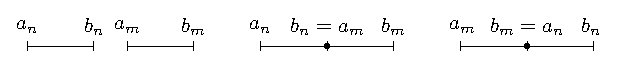
\includegraphics[width=0.65\textwidth]{MA3L12_1.eps}
	\label{MA3L12_1}
	\caption{Расположение отрезков $\Delta_n$ и $\Delta_m$, при $n \neq m$.}
	\label{fig:Покрытие	}
\end{figure}
По-другому это можно записать так: $\mathring{\Delta}_n \cap \mathring{\Delta}_m = \VN, \, \forall n \neq m$, где $\mathring{\Delta}$ означет внутренность интервала $\Delta$. Каждому такому множеству $F$ мы можем приписать длину $\lambda(F)$: 
$$
	\lambda(F) = \sum\limits_{n}|\Delta_n|
$$ 
Порядок нумерования отрезков - не важен, поскольку абсолютно сходящийся ряд не меняет своей суммы от перестановки мест слагаемых. Далее рассматриваем множества только такого вида.
\begin{prop}
	Если $F \subset \displaystyle \bigcup\limits_j F_j$, то $\lambda(F) \leq \displaystyle\sum\limits_{j} \lambda(F_j)$.
\end{prop}
\begin{prop}
	Пусть есть последовательность вложенных множеств: $F_1 \supset F_2 \supset \dotsc \supset F_n \supset \dotsc $. Причем известно, что $\forall n, \, \lambda(F_n) \geq \delta > 0$, тогда пересечение не может быть пустым: $\displaystyle \bigcap\limits_{n} F_n \neq \VN$.
\end{prop}

\end{document}